% fig_flowchart.tex — Fig. 2: Sphere-ICPO algorithm flowchart
% Compile: pdflatex fig_flowchart.tex
\documentclass[tikz,border=10pt]{standalone}
\usepackage{tikz}
\usetikzlibrary{arrows.meta,shapes.geometric,positioning,calc,fit}

\begin{document}
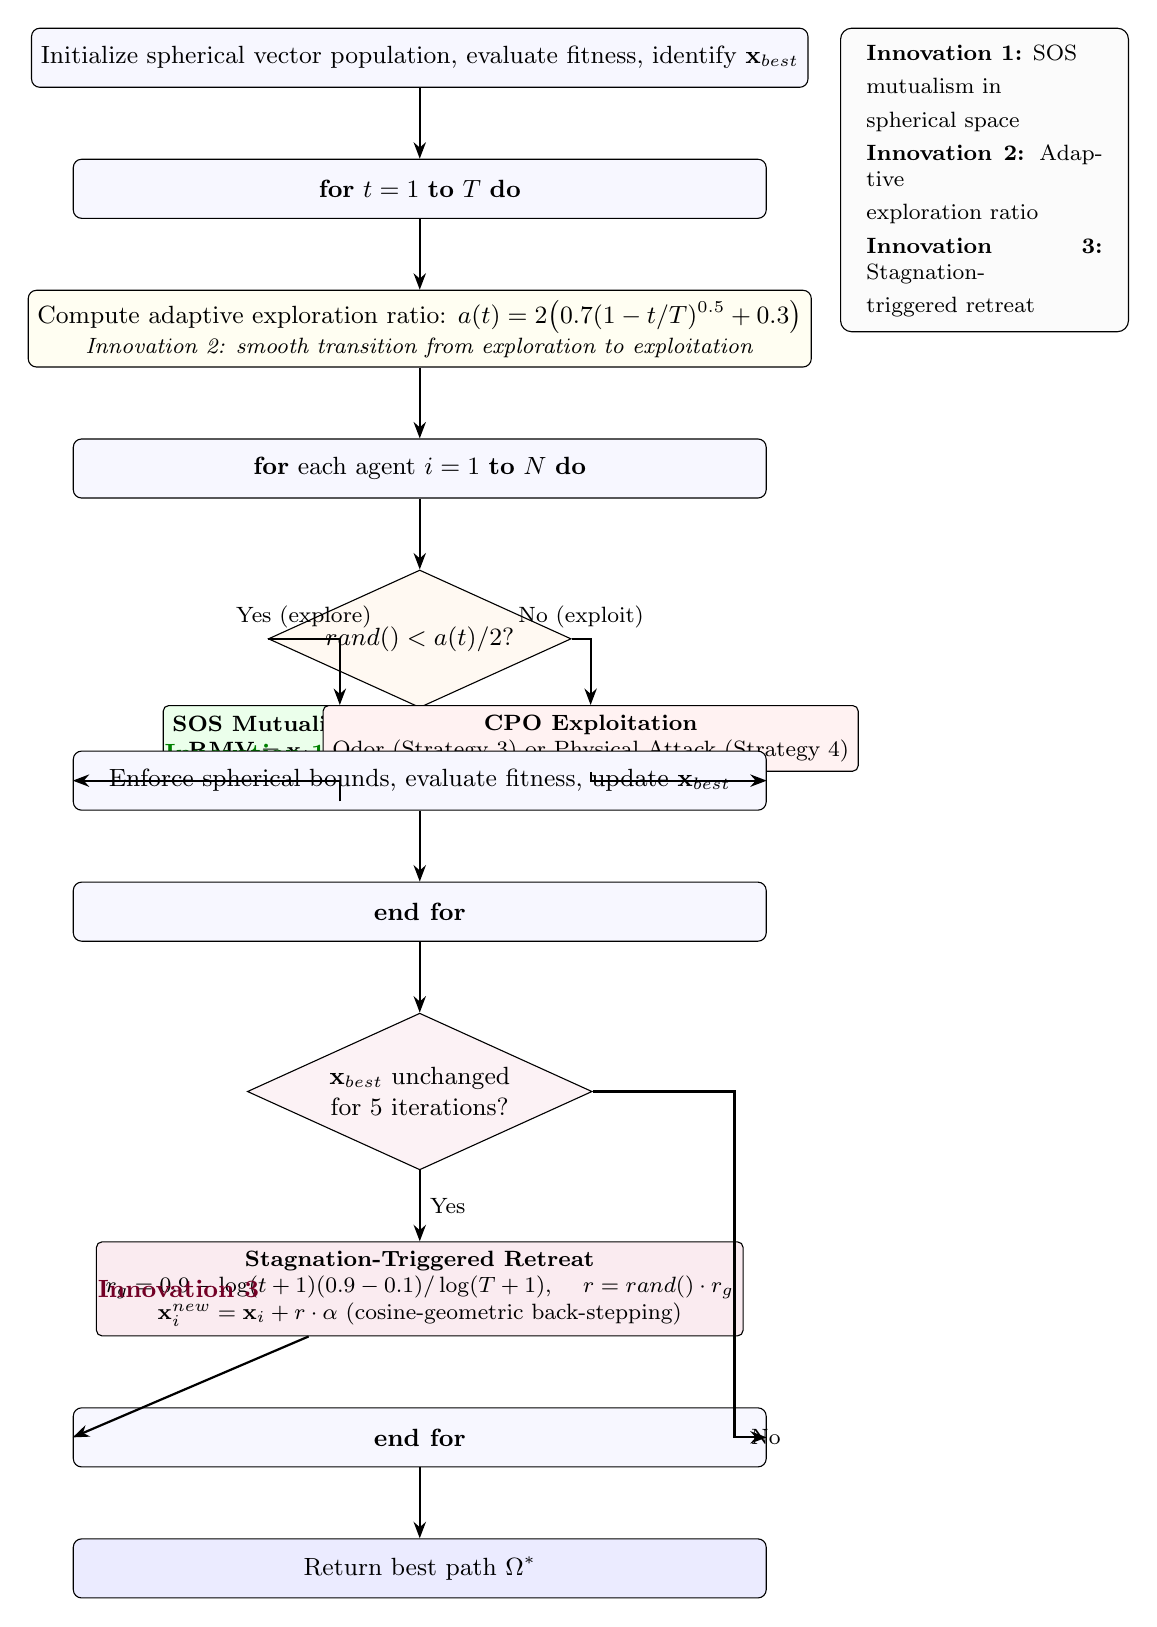
\begin{tikzpicture}[
    node distance=0.9cm,
    block/.style={rectangle,draw,rounded corners=3pt,fill=blue!3,minimum width=8.8cm,minimum height=0.75cm,align=center,font=\small},
    decision/.style={diamond,draw,fill=orange!5,minimum width=3.2cm,minimum height=1.0cm,align=center,font=\small,aspect=2.2},
    subblock/.style={rectangle,draw,rounded corners=2pt,fill=green!5,minimum width=3.8cm,minimum height=0.7cm,align=center,font=\footnotesize},
    arrow/.style={-{Stealth[scale=0.9]},thick},
    label/.style={font=\footnotesize\itshape},
    contrib/.style={font=\footnotesize\bfseries,anchor=west},
]

% ===== START =====
\node[block] (init) {Initialize spherical vector population, evaluate fitness, identify $\mathbf{x}_{\text{best}}$};

% ===== MAIN LOOP =====
\node[block,below=of init] (iter) {\textbf{for} $t = 1$ \textbf{to} $T$ \textbf{do}};

% Compute adaptive a
\node[block,below=of iter,fill=yellow!5] (adapt) {Compute adaptive exploration ratio: $a(t) = 2\bigl(0.7(1 - t/T)^{0.5} + 0.3\bigr)$\\\footnotesize\textit{Innovation 2: smooth transition from exploration to exploitation}};

\node[block,below=of adapt] (agent) {\textbf{for} each agent $i = 1$ \textbf{to} $N$ \textbf{do}};

% Decision
\node[decision,below=of agent] (decide) {$\text{rand}() < a(t)/2$?};

% SOS branch
\node[subblock,below left=0.4cm and -2.2cm of decide,fill=green!8] (sos) {\textbf{SOS Mutualism} (Exploration)\\$\mathbf{RMV} = \mathbf{x}_i + r_1(\mathbf{x}_{\text{rand}} - \mathbf{x}_i)$\\$\mathbf{x}_i^{\text{new}} = \mathbf{x}_i + r_2(\mathbf{x}_{\text{best}} - \mathbf{RMV})$};

% CPO branch
\node[subblock,below right=0.4cm and -2.2cm of decide,fill=red!5] (cpo) {\textbf{CPO Exploitation}\\Odor (Strategy 3) or Physical Attack (Strategy 4)};

% Contribution label for SOS
\node[contrib,green!50!black] at ($(sos.west)+(-0.1,0)$) {\small Innovation 1};

% Merge after branches
\node[block,below=3.2cm of agent] (eval) {Enforce spherical bounds, evaluate fitness, update $\mathbf{x}_{\text{best}}$};
\node[block,below=of eval] (endagent) {\textbf{end for}};

% Stagnation check
\node[decision,below=of endagent,fill=purple!5] (stag) {$\mathbf{x}_{\text{best}}$ unchanged\\for 5 iterations?};

% Retreat
\node[subblock,below=of stag,fill=purple!8,minimum width=7cm] (retreat) {\textbf{Stagnation-Triggered Retreat}\\$r_g = 0.9 - \log(t+1)(0.9-0.1)/\log(T+1)$, \quad $r = \text{rand}() \cdot r_g$\\$\mathbf{x}_i^{\text{new}} = \mathbf{x}_i + r \cdot \alpha$ (cosine-geometric back-stepping)};
\node[contrib,purple!60!black] at ($(retreat.west)+(-0.1,0)$) {\small Innovation 3};

% End loop
\node[block,below=of retreat] (enditer) {\textbf{end for}};

% ===== RETURN =====
\node[block,below=of enditer,fill=blue!8] (ret) {Return best path $\Omega^*$};

% ===== ARROWS =====
\draw[arrow] (init) -- (iter);
\draw[arrow] (iter) -- (adapt);
\draw[arrow] (adapt) -- (agent);
\draw[arrow] (agent) -- (decide);

% Decision branches
\draw[arrow] (decide) -| (sos) node[pos=0.25,above,font=\footnotesize] {Yes (explore)};
\draw[arrow] (decide) -| (cpo) node[pos=0.25,above,font=\footnotesize] {No (exploit)};

% Merge
\draw[arrow] (sos) |- (eval);
\draw[arrow] (cpo) |- (eval);

\draw[arrow] (eval) -- (endagent);
\draw[arrow] (endagent) -- (stag);

% Stagnation branches
\draw[arrow] (stag) -- (retreat) node[midway,right,font=\footnotesize] {Yes};
\draw[arrow] (retreat) -- (enditer.west);
\draw[arrow] (stag.east) -- ++(1.8,0) |- (enditer.east) node[pos=0.6,right,font=\footnotesize] {No};

\draw[arrow] (enditer) -- (ret);

% ===== LEGEND =====
\node[draw,rounded corners,fill=gray!3,anchor=north west,minimum width=3.2cm] at ($(init.north east)+(0.4,0)$) {
    \begin{tabular}{p{3.0cm}}
    \footnotesize\textbf{Innovation 1:} SOS\\
    \footnotesize mutualism in\\
    \footnotesize spherical space\\
    \footnotesize\textbf{Innovation 2:} Adaptive\\
    \footnotesize exploration ratio\\
    \footnotesize\textbf{Innovation 3:} Stagnation-\\
    \footnotesize triggered retreat
    \end{tabular}
};

\end{tikzpicture}
\end{document}
